\documentclass[spanish]{beamer}
\usepackage[ansinew]{inputenc} % Acepta caracteres en castellano
\usepackage[spanish]{babel}    % silabea palabras castellanas
\usepackage{amsmath}
\usepackage{mathtools,cancel} % cancela con una flecha \cancelto{0}{XXXX}
\renewcommand{\CancelColor}{\color{red}} %change cancel color to red
\usepackage{amsfonts}
\usepackage{amssymb}
\usepackage{dsfont}
\usepackage{graphicx}
\usepackage{geometry}
\usetheme{Madrid}
\usecolortheme{beaver}
\usepackage{textpos}
% Logo  en el comienzo 
\addtobeamertemplate{frametitle}{}{%
\begin{textblock*}{100mm}(.85\textwidth,-1cm)
{\includegraphics[height=0.4in, keepaspectratio=true]{/Users/luisnunez/Dropbox/MisDocumentos/UIS/UISImagenInstitucional/UISLOGO.png}}
\end{textblock*}}

\begin{document}

\title{\textbf{Vector Laplace-Runge-Lenz} }
\author[L.A. N��ez]{\textbf{Luis A. N��ez}}  
\institute[UIS]{\textit{Escuela de F�sica, Facultad de Ciencias, } \\
\textit{Universidad Industrial de Santander, Santander, Colombia } \\
{\includegraphics[height=0.4in, keepaspectratio=true]{/Users/luisnunez/Dropbox/MisDocumentos/UIS/UISImagenInstitucional/UISLOGO.png}}
}
\date{\today}
\maketitle


\begin{frame}
\frametitle{Agenda}
  \tableofcontents
\end{frame}


%%%%% Diapo 1
\section{El problema de Kepler y el vector $\mathbf{A}$, Laplace-Runge-Lenz }
\frame{
  \frametitle{El vector $\mathbf{A}$}
   \begin{itemize}  
  	\item<1-> En el problema de Kepler tenemos $V(r)=-k / r$ y  $\mathbf{f}(r) =-k / r^2 \hat{\mathbf{r}}$, 
	\item<2-> La trayectoria es un c�nica, $\frac{q}{r}=1+e \cos \theta$, con $q=L^2 / \mu k$, y $e=\sqrt{1+\frac{2 E L^2}{\mu k^2}}$.
	\item<3-> Definimos el vector de Laplace-Runge-Lenz como: $ \mathbf{A} = \mathbf{p} \times \mathbf{L} - \mu k\hat{\mathbf{r}}$ \\
	\item<4-> Es un vector constante en magnitud y direcci�n. Apunta en la direcci�n del perihelio: \( \mathbf{A} \cdot \mathbf{L} = 0 \): \( \mathbf{A} \) est� en el plano de la �rbita.
	\begin{figure}[t]
		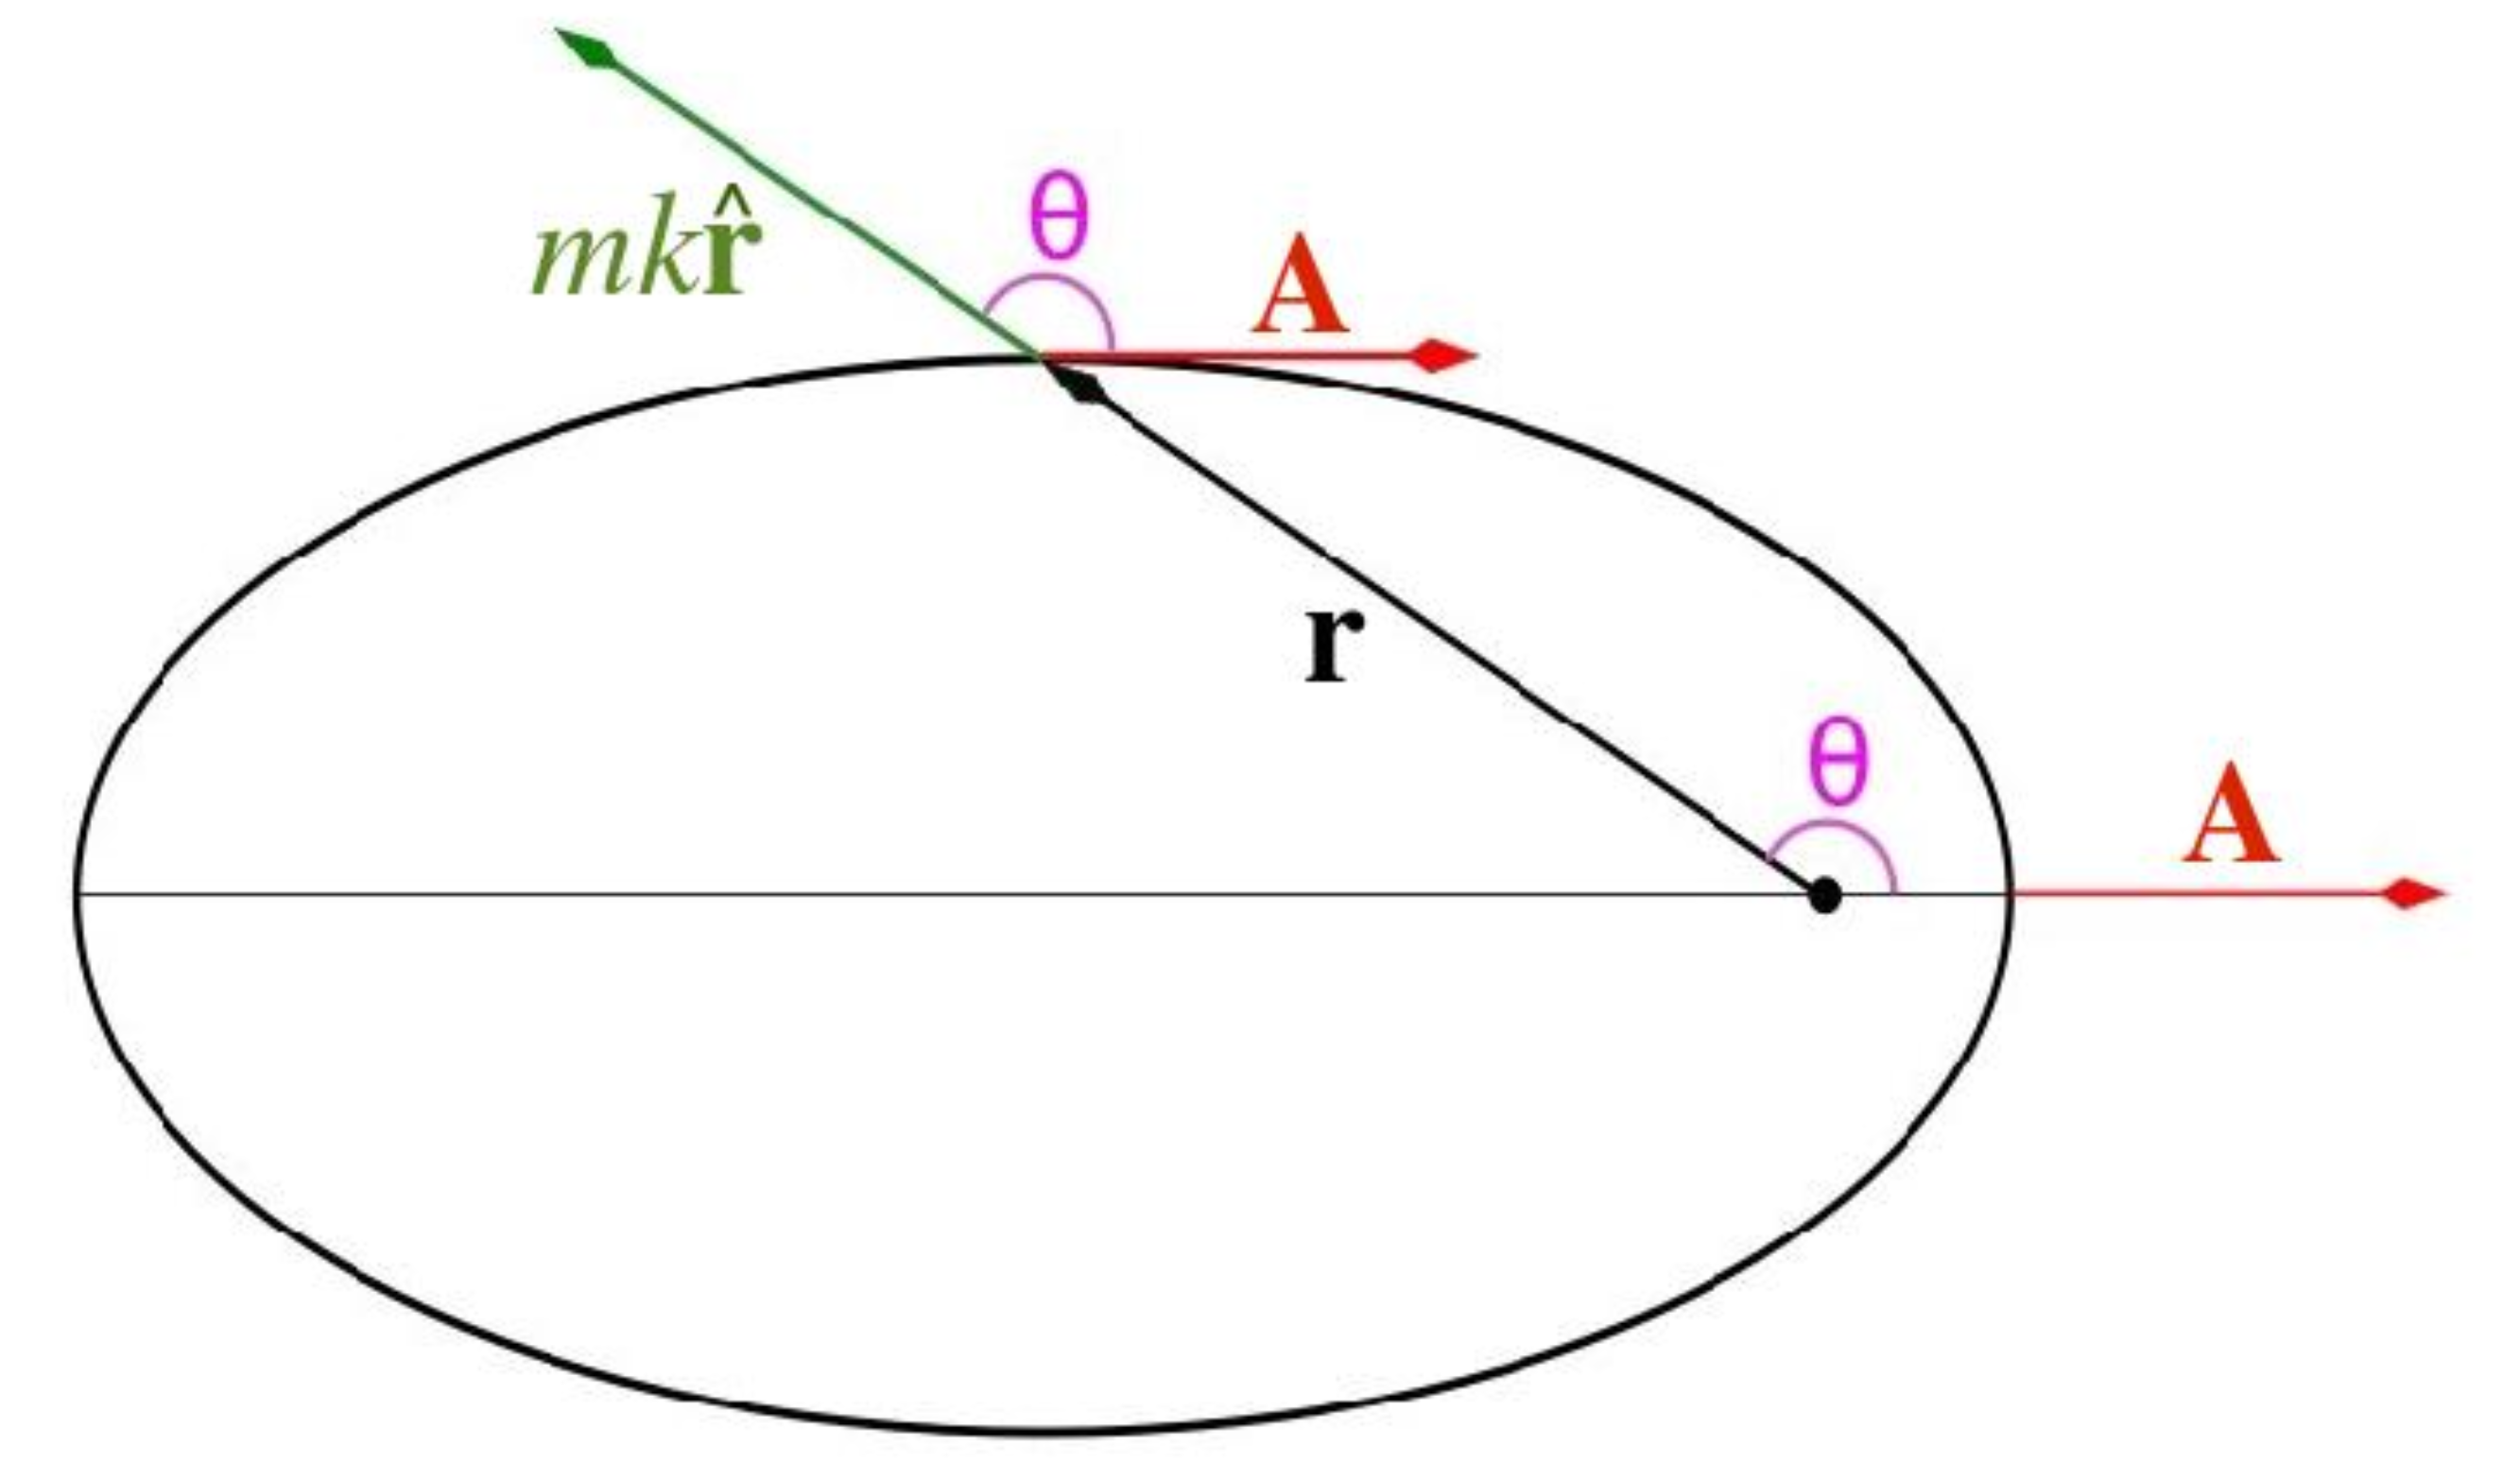
\includegraphics[width=1.8in]{Figuras/VectorA.png}
   	\end{figure}
	\item<5-> Como $L^2=\mathbf{L} \cdot \mathbf{L}=\mathbf{L} \cdot(\mathbf{r} \times \mathbf{p})=\mathbf{r} \cdot(\mathbf{p} \times \mathbf{L}) \Rightarrow \mathbf{r} \cdot \mathbf{A}=\mathbf{r} \cdot[(\mathbf{p} \times \mathbf{L})-\mu k \hat{\mathbf{r}}]$
	\item<6-> Donde $\mathbf{A} \equiv \mathbf{p} \times \mathbf{L} -\mu k \hat{\mathbf{r}}$ y tambi�n $\mathbf{A} \cdot \mathbf{L}=0$
	 
    \end{itemize}
}
%%%%% Diapo 2
\section{El vector $\mathbf{A}$ como cantidad conservada}
\frame{
  \frametitle{$\mathbf{A}$ es cantidad conservada}
   \begin{itemize}  
  	\item<1-> Consideremos $\frac{d \mathbf{A}}{d t}=\frac{d}{d t}(\mathbf{p} \times \mathbf{L})-\mu k \frac{d \hat{\mathbf{r}}}{d t}$
	\item<2-> El primer t�rmino $\frac{d}{d t}(\mathbf{p} \times \mathbf{L})=\frac{d \mathbf{p}}{d t} \times \mathbf{L}+\mathbf{p} \times \cancelto{0}{\frac{d \mathbf{L}}{d t}} =\frac{d \mathbf{p}}{d t} \times(\mathbf{r} \times \mu \mathbf{v})$
	\item<3-> Por otro lado, $\frac{d \mathbf{p}}{d t}=\mathbf{f}(r)=f(r) \hat{\mathbf{r}}=f(r) \frac{\mathbf{r}}{r}$ 
	\item<4-> Entonces $\frac{d}{d t}(\mathbf{p} \times \mathbf{L})=\mu \frac{f(r)}{r}\left[\mathbf{r} \times\left(\mathbf{r} \times \frac{d \mathbf{r}}{d t}\right)\right] = \mu \frac{f(r)}{r}\left[\mathbf{r}\left(\mathbf{r} \cdot \frac{d \mathbf{r}}{d t}\right)-r^2 \frac{d \mathbf{r}}{d t}\right] $ \\ ya que $\mathbf{a} \times(\mathbf{b} \times \mathbf{c})=\mathbf{b}(\mathbf{a} \cdot \mathbf{c})-\mathbf{c}(\mathbf{a} \cdot \mathbf{b})$
	\item<5-> Como $\frac{d}{d t}(\mathbf{r} \cdot \mathbf{r})=2 \mathbf{r} \cdot \frac{d \mathbf{r}}{d t}=\frac{d}{d t}\left(r^2\right)=2 r \frac{d r}{d t}$ 
	\item<6-> Tendremos $\frac{d}{d t}(\mathbf{p} \times \mathbf{L})=\mu f(r)\left[\mathbf{r} \frac{d r}{d t}-r \frac{d \mathbf{r}}{d t}\right]$
	\item<7-> Adem�s $\frac{d}{d t}\left(\frac{\mathbf{r}}{r}\right)  =\frac{d \mathbf{r}}{d t} \frac{1}{r}-\frac{\mathbf{r}}{r^2} \frac{d r}{d t} \Rightarrow \quad-r^2 \frac{d}{d t}\left(\frac{\mathbf{r}}{r}\right)  =\mathbf{r} \frac{d r}{d t}-r \frac{d \mathbf{r}}{d t}$
	\item<8-> Con lo cual $\frac{d}{d t}(\mathbf{p} \times \mathbf{L})=-\mu f(r) r^2 \frac{d}{d t}\left(\frac{\mathbf{r}}{r}\right) = \mu k \frac{d}{d t}\left(\frac{\mathbf{r}}{r}\right)=\mu k \frac{d \hat{\mathbf{r}}}{d t}$ para $f(r)=-k / r^2$
	\item<9-> y finalmente $\frac{d \mathbf{A}}{d t}=0 \Rightarrow \mathbf{A} \equiv \mathbf{p} \times \mathbf{L} -\mu k \hat{\mathbf{r}} =$cte
	\item<10-> La magnitud del vector \textbf{A} para la fuerza gravitacional se expresa en t�rminos de $L$ y $E$ como $A^2=(\mu k e)^2=\mu^2 k^2+2 \mu E L^2=$ cte
\end{itemize}
}

%%%%% Diapo 2
\section{Problema Kepler superintegrable}
\frame{
\frametitle{Kepler superintegrable}
\begin{itemize}  
	\item<1-> La direcci�n de $\mathbf{A}$, correspondiente a la direcci�n del perihelio, provee una nueva cantidad conservada en el problema de Kepler.
	\begin{figure}[t]
		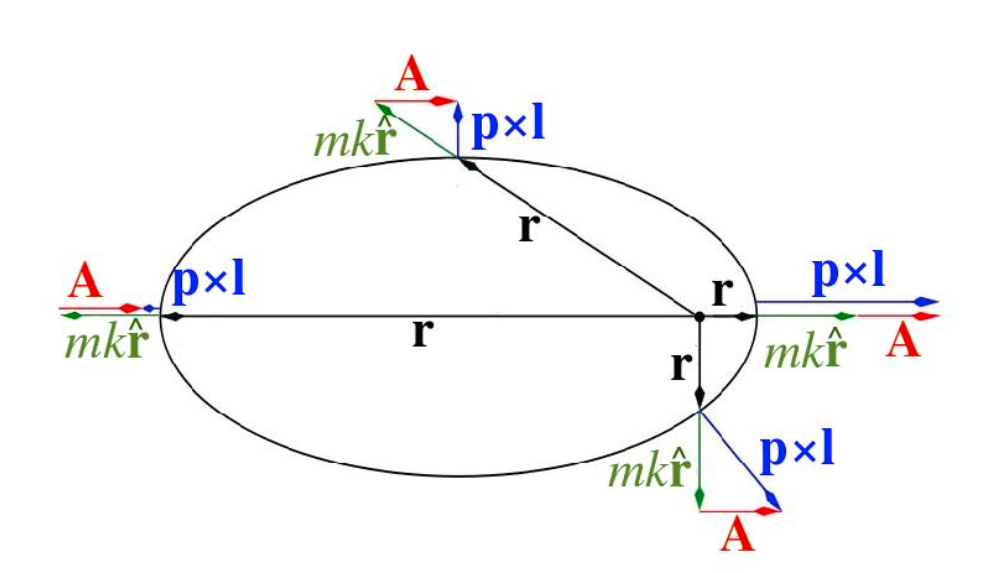
\includegraphics[width=1.8in]{Figuras/DirA.png}
   	\end{figure}
	\item<2->La direcci�n $\hat{\mathbf{A}}$ constante implica que la �rbita para $V(r)=-k / r$ no  precesa.
	\item<3-> El sistema de dos cuerpos sujetos a la fuerza gravitacional que var�a como el inverso del cuadrado de la distancia constituye un sistema superintegrable. 
	\item<4-> Existen seis grados de libertad (tres para cada part�cula) y siete cantidades conservadas: las tres componentes de la velocidad del centro de masa $\mathbf{v}_{c m}$, la direcci�n del momento angular $\mathbf{L}$, su magnitud $L$, la energ�a $E$ y la direcci�n del vector de Laplace-Runge-Lenz $\hat{\mathbf{A}}$
\end{itemize}
}

%
%%%%% Diapo 2
\section{Spoiler Alert. Simetr�as Escondidas y par�ntesis de Poisson}
\frame{
\frametitle{Simetr�as Escondidas y par�ntesis de Poisson 1/2}
\begin{itemize}  
	\item<1-> Mas adelante en este curso, si tenemos un sistema de $n$ part�culas libres, definiremos el espacio de configuraciones como un espacio de $3n$ dimensiones $(r_{x\,k}, r_{y\,k}, r_{z\,k})$, con $i= 1, 2, \cdots, n$ 
	\item<2-> Ese mismo sistema de part�culas libres lo podremos describir en el espacio de fases de $6n$ dimensiones $(q_k , p_{k})$ con $k= 1, 2, \cdots, 3n$
	\item<3-> En el espacio de fases definiremos los par�ntesis de Poisson para dos funciones  \( f, g \) cualesquiera:$\{f, g\} = \sum_i \left( \frac{\partial f}{\partial q_i} \frac{\partial g}{\partial p_i} - \frac{\partial f}{\partial p_i} \frac{\partial g}{\partial q_i} \right)$
	\item<4-> Sea una funci�n $f\left(q_i, p_i, t\right)$ en el espacio de fase $\left(q_i, p_i\right)$, $i=1, \ldots, s$, de un sistema mec�nico con una funci�n energ�a $\mathcal{E}=\mathcal{H}\left(q_i, p_i, t\right)$ que lo llamaremos Hamiltoniano.
	\item<5-> Entonces $\frac{d f}{d t}=\sum_{i=1}^s\left(\frac{\partial f}{\partial q_i} \dot{q}_i+\frac{\partial f}{\partial p_i} \dot{p}_i\right)+\frac{\partial f}{\partial t} =\{f, \mathcal{H}\}+\frac{\partial f}{\partial t} $.
	\item<6-> Donde $\dot{q}_i=\frac{\partial \mathcal{H}}{\partial p_i}, \quad \dot{p}_i=-\frac{\partial \mathcal{H}}{\partial q_i}$ son las ecuaciones de Hamilton.
	\item<7-> Si $f$ no depende expl�citamente del tiempo $\frac{\partial f}{\partial t}=0$ y es una cantidad conservada $\frac{d f}{d t}=0$, entonces $\{f, \mathcal{H}\}=0$.
\end{itemize}
}
%
%%%%% Diapo 2
\subsection{Dos ejemplos}
\frame{
\frametitle{Dos Ejemplos}
\begin{itemize}  
	\item<1-> Calcular $\{r, \mathbf{p}\}$, donde $r=\left(x^2+y^2+z^2\right)^{1 / 2}$
	\begin{itemize}
		\item $\{r, \mathbf{p}\}=\left\{r, p_x\right\} \hat{\mathbf{x}}+\left\{r, p_y\right\} \hat{\mathbf{y}}+\left\{r, p_z\right\} \hat{\mathbf{z}}$
		\item $\left\{r, p_x\right\}=\sum_{i=1}^3\left(\frac{\partial r}{\partial q_i} \frac{\partial p_x}{\partial p_i}-\frac{\partial r}{\partial p_i} \frac{\partial p_x}{\partial q_i}\right)=\frac{\partial r}{\partial x} \frac{\partial p_x}{\partial p_x}=\frac{x}{r}$
		\item $\left\{r, p_y\right\}=\frac{y}{r}, \quad\left\{r, p_z\right\}=\frac{z}{r}$
		\item luego $\{r, \mathbf{p}\}=\frac{x}{r} \hat{\mathbf{x}}+\frac{y}{r} \hat{\mathbf{y}}+\frac{z}{r} \hat{\mathbf{z}}=\frac{\mathbf{r}}{r}=\hat{\mathbf{r}} $
	\end{itemize}
	\item<2->  Dadas las componentes del momento angular $\mathbf{L}=\mathbf{r} \times \mathbf{p}$:
	$L_x=y p_z-z p_y, \quad L_y=z p_x-x p_z, \quad L_z=x p_y-y p_x$ \\
	Calcular los par�ntesis de Poisson para las componentes de {\bf p} y {\bf L}: \\ 	
	$\left\{p_y, L_x\right\}=-\frac{\partial L_x}{\partial y}=-p_z$;  $\quad \left\{p_x, L_x\right\}=-\frac{\partial L_x}{\partial x}=0$; $\quad \left\{p_z, L_y\right\}=-\frac{\partial L_y}{\partial z}=-p_x$ \\
 $\left\{L_x, L_y\right\} =\sum_{i=1}^3\left(\frac{\partial L_x}{\partial q_i} \frac{\partial L_y}{\partial p_i}-\frac{\partial L_x}{\partial p_i} \frac{\partial L_y}{\partial q_i}\right)$ \\$ 
		\left\{L_x, L_y\right\} = \left(\frac{\partial L_x}{\partial x} \frac{\partial L_y}{\partial p_x}-\frac{\partial L_x}{\partial p_x} \frac{\partial L_y}{\partial x}\right)+\left(\frac{\partial L_x}{\partial y} \frac{\partial L_y}{\partial p_y}-\frac{\partial L_x}{\partial p_y} \frac{\partial L_y}{\partial y}\right)+\left(\frac{\partial L_x}{\partial z} \frac{\partial L_y}{\partial p_z}-\frac{\partial L_x}{\partial p_z} \frac{\partial L_y}{\partial z}\right)$ \\
	$\left\{L_x, L_y\right\} =x p_y-y p_x=L_z$; $\quad \left\{L_y, L_z\right\}  =L_x$ $\quad \left\{L_z, L_x\right\}  =L_y$
	\item<3-> 	Entonces, $\left\{L_i, L_j\right\}=\epsilon_{i j k} L_k$. En Mec�nica Cu�ntica,  $\left[L_i, L_j\right]=i \hbar \epsilon_{i j k} L_k$.	
\end{itemize}
}
%
%%%%% Diapo 2
\section{Spoiler Alert: Simetr�as Escondidas y el Vector de Runge-Lenz}
\frame{
\frametitle{El Vector de Runge-Lenz}
Para un sistema de Kepler en coordenadas cartesianas
\begin{itemize}  
	\item<1-> El Hamiltoniano es $\mathcal{H} = \frac{\vec{p}^2}{2m} - \frac{k}{|\vec{r}|}$
	\item<2-> El vector de Runge Lenz es $\vec{A} = \vec{p} \times \vec{L} - mk \frac{\vec{r}}{r}$
	\item<3-> Muestre que $\frac{d\vec{A}}{dt} = \{\vec{A}, H\} = \{A_i, H\} = 0$, donde las $A_i$ son las componentes cartesianas del vector de Runge-Lenz
	\item<4-> Si $L_k$ son las componente cartesianas de la cantidad de movimiento angular, muestre que $\{L_i, L_j\} = \varepsilon_{ijk} L_k$.  Esta operaci�n define el �lgebra de Lie de SO(3) que garantiza simetr�a rotacional.
	\item<5-> Muestre tambi�n $\{L_i, A_j\} = \varepsilon_{ijk} A_k$
	\item<6-> Adicionalmente, muestre que $\{L_i, A_j\} = \varepsilon_{ijk} A_k$
	\item<7-> El problema de Kepler tiene un grupo de simetr�a ampliado: No s�lo rotaciones espaciales SO(3), sino SO(4) para el caso de �rbitas acotadas, generada por \( \{L_i, \tilde{A}_j\} \)
\end{itemize}
}
 
\end{document}
